\chapter{Sensitivity of the SuperNEMO demonstrator to the $\zeronu$}
\label{ch:sensitivity}

In this chapter, we present the SuperNEMO sensitivity to the search of $\zeronu$ decay, and the corresponding effective neutrino masses, for several isotopes.
The SuperNEMO final detector is expected to exclude Selenium-$82$ $\zeronu$ half-lives up to $1.2\times 10^{26}$ y ($90\%$ CL) if $\zeronu$ decays through the exchange of a light Majorana neutrino, with a detector exposure of $500$ kg.y \cite{art:SuperNEMO2010}.
The sensitivity is given as a limit, in case we do not observe the expected signal.
In $2015$ began the demonstrator installation at the Laboratoire Souterrain de Modane.
With an exposure of $17.5$ kg.y, the demonstrator could set a limit on the $\zeronu$ process of $5.3\times 10^{24}$ y ($90\%$ CL) \cite{CalvezThesis}.

This study aims to explore the impact on the sensitivity of the presence of a magnetic field, and will participate in the final decision on the installation of the coil.
In a context of investigating the demonstrator and final detector capabilities, different internal source contamination levels are explored.
The topology of interest is the two electrons topology, and we use the $2e$ energy sum to discriminate the signal from the background events.
Thanks to SuperNEMO tracking capabilities, topological informations are exploited to improve the SuperNEMO sensitivity.



\section{Signal and background simulations}
\label{sec:sensitivity_simus}

A full simulation for the SuperNEMO demonstrator was performed, in order to determine the longest $\zeronu$ half-life that can be probed with SuperNEMO using the distribution of the sum of electron energies, in the case where the $\zeronu$ decay was not observed.
In the Tab.~\ref{tab:sensitivity_simulations} is summarised the expected number of signal and background events, both for the SuperNEMO demonstrator and final detector, and we present the amount of Monte-Carlo simulations for each isotope.
\begin{table}[h]
  \centering
  \begin{tabular}{|c|cc|c|}
    \hline
    &\multicolumn{2}{c|}{Expected decays} & Simulated decays \\
    & Demonstrator & Final detector & \\
    \hline\hline
    $\zeronu$ ($\Tbeta = 2.5\,10^{23}$ y)~\cite{art:NEMO2018} & $3.6\,10^{2}$ & $1.0\,10^{4}$ & $1.0\,10^{7}$ \\
    $\twonu$ & $9.5\,10^{5}$ & $2.7\,10^{7}$ & $1.0\,10^{7}$ \\
    \Tl  & $5.5\,10^{3}$ & $1.6\,10^{5}$ & $1.0\,10^{7}$ \\
    \Bi  & $1.1\,10^{3}$ & $3.1\,10^{4}$ & $1.0\,10^{7}$ \\
    \Rn  & $1.8\,10^{5}$ & $7.2\,10^{6}$ & $1.0\,10^{7}$ \\
    \hline
  \end{tabular}
  \caption{Expected and simulated decays for different processes, both for the demonstrator ($17.5$ kg.y) and for the final detector ($500$ kg.y), assuming target background activities are reached.
    The $\Tbeta$ value is given only illustratively: the decay has never been observed, so we choose the limit on the half-life obtained with NEMO-$3$~\cite{art:NEMO2018}.
    Expected number of events are given not taking into account the cut efficiencies, and in the full energy range.
    We remind the target activities: $\mathcal{A}^{\text{Tl}} = 10\,\mu$Bq.kg$^{-1}$, $\mathcal{A}^{\text{Bi}} = 2\,\mu$Bq.kg$^{-1}$, $\mathcal{A}^{\text{Rn}} = 0.15$ mBq.m$^{-3}$
    \label{tab:sensitivity_simulations}}
\end{table}


\subsubsection*{The $\zeronu$ signal}

In the following, the assumed underlying mechanism for the $\zeronu$ decay occurs through the exchange of a light Majorana neutrino, the so-called mass mechanism (MM), as it is the most natural and widespread mechanism.
The hypothetical $\zeronu$ signal would be detected as an excess of events in the region of interest, with respect to the predicted background contamination level.
The $10^{7}$ $\zeronu$ Monte-Carlo events are generated using the DECAY$0$ software~\cite{art:decay0}.
The simulations are normalised assuming a $\Tbeta = 6.0\,10^{24}$ y half-life [citation].

\subsubsection*{Inside detector backgrounds}

In the full energy range, the allowed $\twonu$ decay stands as the dominant internal background type.
However, beyond a certain value in energy, the number of $\twonu$ events decreases very quickly, because of the energy spectrum shape.
Moreover, its contribution is reduced if the half-life increases, and is enhanced if the energy resolution is worsened.
To offset this effect, we simulated $10^{7}$ $\twonu$ decays inside the source foils, with a total energy $>2$ MeV, in addition of the normal $\twonu$ decays.
($\Ttwonu = 9.39 \pm 0.17$ (stat) $\pm 0.58$ (syst) $\times 10^{19}$ years from the NEMO-$3$ experiment~\cite{art:NEMO2018}), and we normalised the total $\twonu$ spectrum.
As described in Sec.~\ref{subsec:SNbkg_internal}, source foil contaminations by isotopes such as \Tl\ or \Bi\ constitute the principal internal backgrounds with the $\twonu$ decay.
These backgrounds are processed by the same detector simulation as the $\zeronu$ signal, using DECAY$0$.
Since internal backgrounds have very low efficiencies in the $2e$ topology, we simulated an important amount of Monte-Carlo events.

A component of the external background producing events similar to the internal background is caused by the presence of \Rn\ inside the tracking detector volume, and constitute a separate background category.
\Bi\, being a progeny of \Rn\, can decay on, or near a foil, and appear with a $2e$ topology, becoming hard to distinguish from a double beta decay candidate.
This isotope being distributed throughout the whole tracking detection volume, it was therefore necessary to simulate a large quantity of this isotope in the detector to maximise the amount of \Bi\ events, coming from \Rn\ decays, in the region of interest.

The target background activities detailed in Sec.~\ref{sec:SNbkg} were defined so that each background has a similar contribution to that of the $\twonu$ in the region of interest~\cite{internal:SNphysicsCase}.
We remind these nominal in Tab.~\ref{tab:real_target_act}, and give a comparison with the measured activities of the demonstrator source foils contaminations, as well as a measurement of the \Rn\ activity inside the tracker volume.
\begin{table}[h]
  \centering
  \begin{tabular}{|c|c|c|}
    \hline
    & Nominal activities & Real activities \\
    \hline\hline
    \Tl  & $10\,\mu$Bq.kg$^{-1}$ & $54\,\mu$Bq.kg$^{-1}$ \\
    \Bi  & $2\,\mu$Bq.kg$^{-1}$ & $<290\,\mu$Bq.kg$^{-1}$ \\
    \Rn  & $0.15$ mBq.m$^{-3}$ & $0.15\pm 0.02$ mBq.m$^{-3}$~\cite{conf:radon2017} \\
    \hline
  \end{tabular}
  \caption{Real and targeted nominal activities for the SuperNEMO detector.
  \label{tab:real_target_act}}
\end{table}


\subsubsection*{Outside detector backgrounds}

This background category is due to the external $\gamma$-ray flux produced by radioactive isotope decays in detector components or surrounding laboratory rocks, as well as neutron interactions in the shield and of the detector's material.
The limit on external background number of counts set by the NEMO-$3$ experiment was $<0.2$ in the $2e$ total energy range [$2.8$;$3.2$] MeV, for an exposure of $34.3$ kg·y with $^{100}$Mo ~\cite{art:NEMO2015}.
The most notorious difference is the fact that the SuperNEMO scintillator blocks are thicker than those of NEMO-$3$.
Therefore, a gamma is less likely to cross a scintillator without interacting, and we can reject it if an interaction occurs.
As a consequence, for the same PMTs radioactivity, the gamma background rate is less important for the SuperNEMO demonstrator than for NEMO-$3$.
Moreover, radiopurity measurement for SuperNEMO PMTs allow to conclude that the total activity of SuperNEMO PMTs is better than for NEMO-$3$, for the two principal considered isotopes \Tl\ and \Bi ~\cite{docdb:perrot2017}.
Thus, it is justified to consider that all external backgrounds from outside the foil, apart from \Rn\ in the tracking volume, are expected to be negligible, and were not simulated.
Nevertheless, it is important to note that the energy window for SuperNEMO starts at $2.7$ MeV, and not at $2.8$ MeV as for NEMO-$3$, which could be a cause of increase in external background.

We select only events matching the $2e$ topology.
A reconstructed particle is tagged as an electron if it has a negatively curved track with a vertex on the source foils and an associated calorimeter hit.
All these represent what we call \emph{the first order cuts}.
In the following we present an optimisation of the event selection that have been set up to maximise the signal over background ratio.

%% \begin{itemize}
%% \item Justifier bdf externe avec article nemo3 (plus diff roi et meilleure eff)
%% \item The dominant two neutrino $\twonu$ background and the background due to foil contaminations were normalised assuming a demonstrator exposure of $17.5$ kg.y.
%% \item The total energy brought by the two electrons is a continuum presenting a reduced number of events in the region of interest, due to electron energy losses before reaching the calorimeter (mainly inside the dense source material, as well as inside the wire chamber).
%% \end{itemize}


\section{Optimisation of event selection}
\label{sec:sensitivity_ev_selection}

Most of the double beta experiments are only sensitive to the total electron energy sum.
SuperNEMO, coupling tracking and calorimetry technologies, is sensitive to individual energies and the angle between the two electrons, which gives it the ability to individually consider both electrons, thereby evaluating whether the two particles were emitted simultaneously from the same vertex or not.
To allow the selection of $\zeronu$ signal events while rejecting a high proportion of background events, topological cuts have been set up, in addition with the basic first order cuts described above.
\begin{itemize}
\item \Pint\ $>4\%$:\\
  The internal probability, based on time-of-flight (TOF) computation, is detailed in Sec.~\ref{subsec:internal_prob}.
  The chosen level insures that non simultaneous events are rejected.
\item $\Delta y < 60$ mm and $\Delta z < 70$ mm:\\
  The two reconstructed vertices on source foils should not be separated by more than $60$ mm horizontally, and by more than $70$ mm vertically, to maximise the selection of two electrons emitted at the same spot.
\end{itemize}
These cuts follow the NEMO-$3$ analysis on the external background rejection, whose effectiveness were lately confirmed for the SuperNEMO demonstrator~\cite{docdb:calvez2014}.
First order and topological cuts have an efficiency of selection that differs for each decays.
These efficiencies are presented in Tab.~\ref{tab:selections_eff}.
\begin{table}[h]
  \centering
  \begin{tabular}{|c|c|c|c|}
    \hline
    & First order cuts (\%) & Internal probability (\%) & Vertex distance (\%)  \\
    \hline\hline
    $\zeronu$  & $26.9$ & $25.3$ & $24.2$ \\
    $\twonu$  & $9.16$ & $8.57$ & $8.01$ \\ %% (à recalculer avec 2nu2mev)
    \Tl  & $0.106$ & $0.0888$ & $0.0821$\\
    \Bi  & $0.168$ & $0.151$ & $0.140$ \\
    \Rn  & $0.0169$ & $7.3\times 10^{-5}$ & $4.27\times 10^{-5}$\\
    \hline
  \end{tabular}
  \caption{Number of selected $2e$ topologies compared with the total number of simulated decays, for first order cuts and topological cuts.
  \label{tab:selections_eff}}
\end{table}
Topological cuts are designed to reject events where the two electrons are not emitted simultaneously, or from the same location on the source foil, and hence decreases the number of expected events for all the backgrounds but especially for Radon.
As explained in Sec.~\ref{sec:sensitivity_simus}, the \Bi decays following a Radon contamination of the tracker are not emitted from the source, but mainly from the tracker wires.
The internal probability and vertices separation can therefore help discriminate such events from signal events.

We present the total energy spectra for each simulated process, after event selection, in Fig.~\ref{fig:sensitivity_energy_spectra}.
\begin{figure}[h]
\centering
\begin{subfigure}[t]{0.48\textwidth}
  \centering
  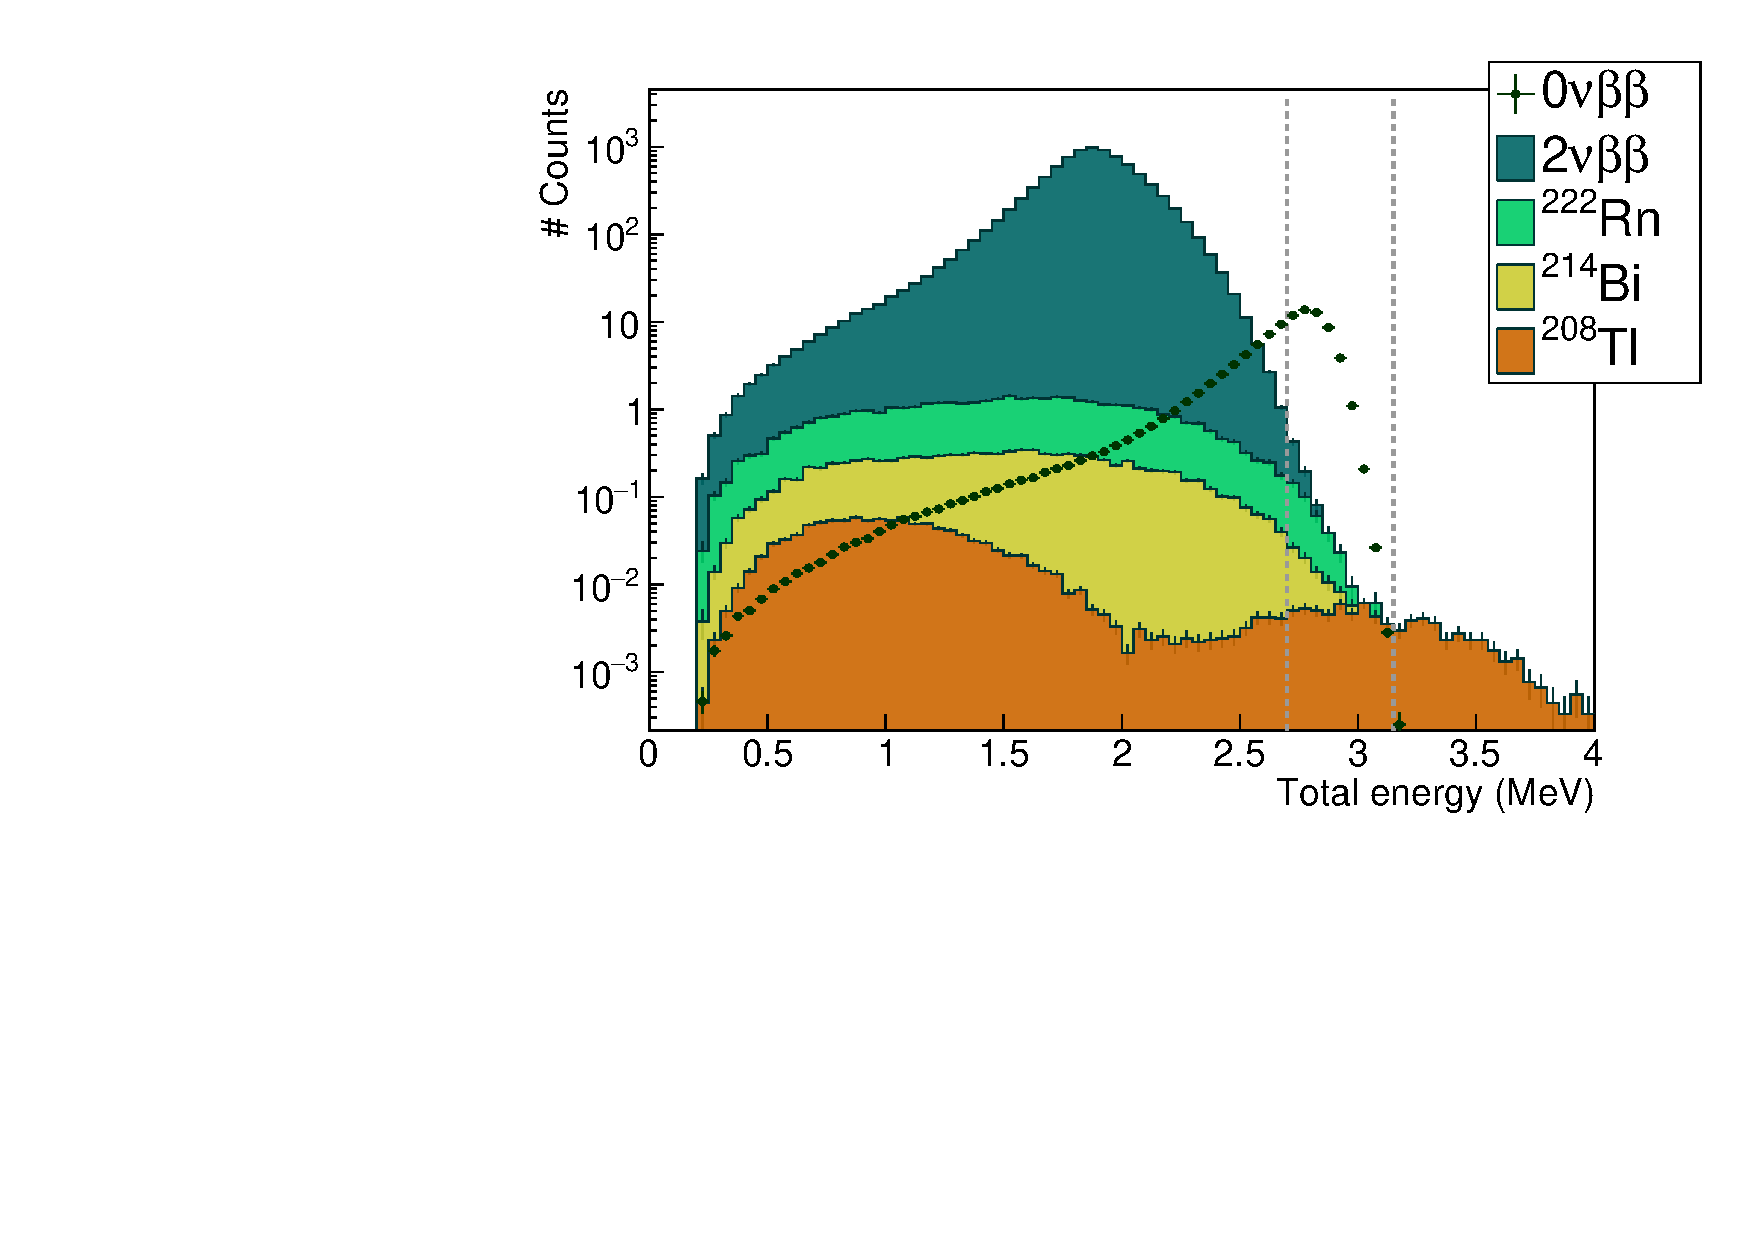
\includegraphics[width=1.1\textwidth]{Sensitivity/fig_sensitivity/energy_spectrum_with_B_82Se.pdf}
  \captionsetup{justification=centering}
  \caption{
    \label{subfig:sensitivity_energy_spectra_full}}
\end{subfigure}
\hfill
\begin{subfigure}[t]{0.48\textwidth}
  \centering
  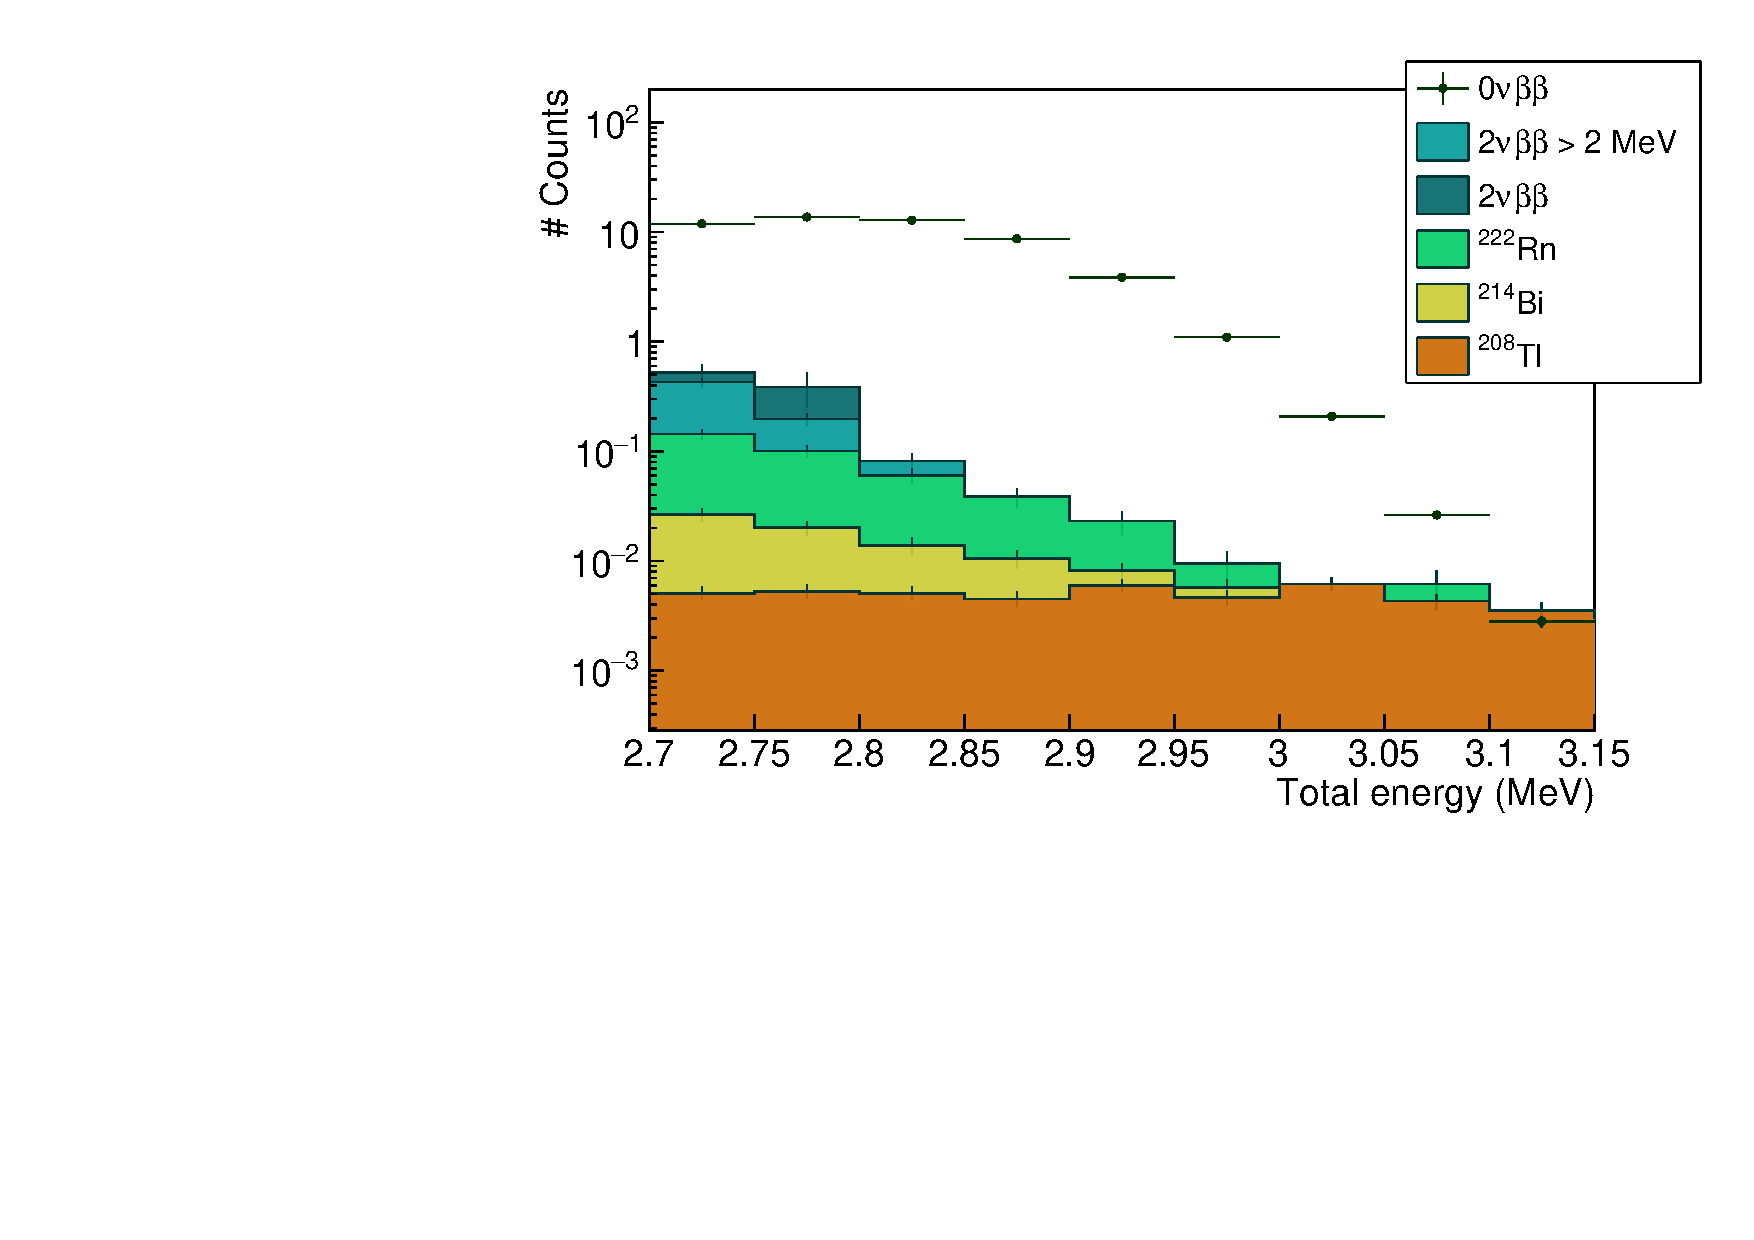
\includegraphics[width=1.1\textwidth]{Sensitivity/fig_sensitivity/energy_spectrum_with_B_82Se_zoom.pdf}
  \captionsetup{justification=centering}
  \caption{
    \label{subfig:sensitivity_energy_spectra_zoom}}
\end{subfigure}
\caption{Total energy spectra for the $\zeronu$ signal and main backgrounds, for (a) the full energy range, and (b) for the [$2.7$;$3.2$] MeV energy range, whose optimisation is discussed in Sec.~\ref{sec:Nbkg_ROI}.
  \label{fig:sensitivity_energy_spectra}}
\end{figure}
% The total number of events for each decay represent the amount of selected $2e$ topologies.
The $\zeronu$ spectrum is peaked around $2.8$ MeV, as the available energy $\Qbb = 2.99$ MeV is degraded by electron energy losses before reaching the calorimeter (mainly inside the dense source material, as well as inside the wire chamber), explaining the asymmetric energy distribution.
% The progeny of \Rn\ produces $\gamma$-rays and $\beta$ decays accompanied by internal conversion (IC), Møller or Compton scattering, the dominant mechanism being the first one.
\Bi\ being one of the descendants of \Rn, their energy distributions follow the same variations, except that a high part of \Rn\ events inside the tracker have been rejected by the topological cuts.
The \Tl\ energy distribution reveals the internal conversion of the $2.6$ MeV gamma, emitted after \Tl\ $\beta^{-}$ disintegrations.

In the following section, we give informations about the expected number of background events, especially in the region of interest.

\section{Expected number of background events and optimisation of the region of interest}
\label{sec:Nbkg_ROI}

As the two electrons energy sum for the possible $\zeronu$ is a peak (enlarged by electron energy losses and calorimeter energy resolution), it is interesting to constraint the $\zeronu$ decay searches to a given energy range, the so-called \emph{region of interest} (ROI).
In the following, we expose how the search for the best limit on $\Tbeta$ is a guide to determine the best ROI.
%The optimisation of this energy window consists of cutting the full energy range in several sub-ranges, and compute the selection efficiencies for all energy sub-ranges.

For a given energy range, the $\zeronu$ half-life depends on the signal detection efficiency $\epsilon$ in this energy window, on the limit on expected signal events $N_{\text{expected}}$, as well as on the source isotope nature and the detector's exposure $m\times t$, following
\begin{equation}
  \Tbeta > \frac{\mathcal{N}_{\text{A}}\log{2}}{M}\times \frac{\epsilon\times m\times t}{N_{\text{expected}}}\,,
  \label{eq:tbeta_limit}
\end{equation}
with $\mathcal{N}_{\text{A}}$ the Avogadro number and $M$ the source isotope's molar mass.
The half-life is given as a limit, in case we do not observe the expected signal.
In order to evaluate $N_{\text{expected}}$, and later the demonstrator's sensitivity to the $\zeronu$ decay, we must determine the number of background events occurring in the region of interest.
This calculation, for a given energy window, differs with the background type.
\begin{itemize}
\item The $\twonu$ background\\
  The number of $\twonu$ events $N_{2\nu}$ depends, in addition to the exposure, on the number of atoms composing the source foils, on the $\twonu$ decay half-life $\Ttwonu$, and on $\epsilon_{2\nu}$ the selection efficiency for the $\twonu$ process, as
  \begin{equation}
    N_{2\nu} = \frac{\mathcal{N}_{\text{A}}\log{2}}{M}\times\frac{\epsilon_{2\nu}\times m\times t}{\Ttwonu}\,.
  \end{equation}
\item Natural radioactive internal backgrounds (\Tl\ and \Bi)\\
  Considering $A_{\text{int}}$ as the internal background activities, and $\epsilon_{\text{int}}$ their selection efficiencies in a given energy window, the number of background events emitted from the source is
  \begin{equation}
    N_{\text{int}} = A_{\text{int}}\epsilon_{\text{int}}\times m\times t\,.
  \end{equation}
\item Radon background\\
  The same way, we can define the number of radon events occurring in the whole tracker volume $V = 15.3$ m$^{3}$ as
  \begin{equation}
    N_{\text{Rn}} = A_{\text{Rn}}\epsilon_{\text{Rn}}\times V\times t\,.
  \end{equation}
\end{itemize}
The cumulative efficiency spectra, computed by comparing the number of selected events to the number of Monte-Carlo events in $E>E_{\text{min}}$ energy ranges, are presented in Fig.~\ref{subfig:sensitivity_efficiency_spectra}.
Once computed, the efficiency of selection helps finding the number of background events expected, displayed in Fig.~\ref{subfig:sensitivity_Nbkg_spectra}.
\begin{figure}[h]
\centering
\begin{subfigure}[t]{0.48\textwidth}
  \centering
  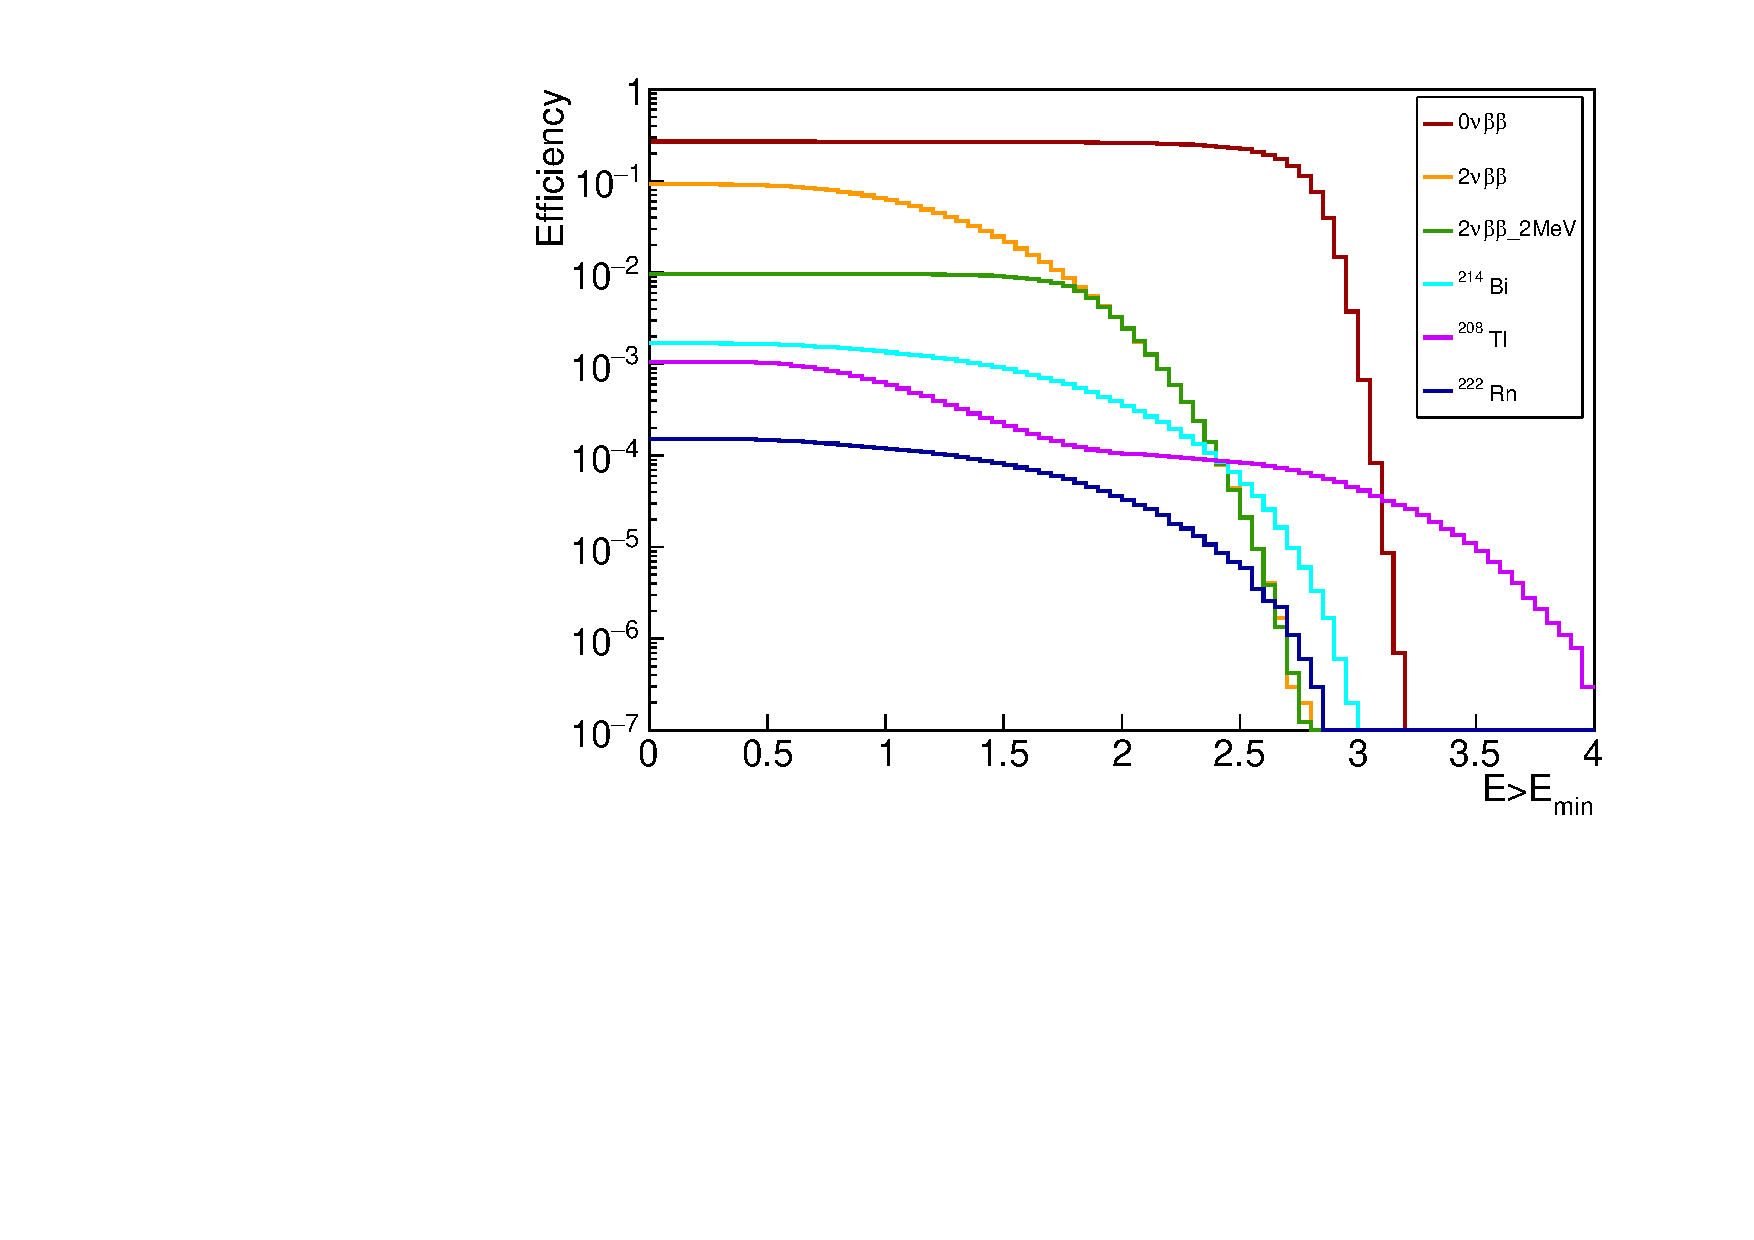
\includegraphics[width=1.1\textwidth]{Sensitivity/fig_sensitivity/efficiency_spectrum_with_B_82Se.pdf}
  \captionsetup{justification=centering}
  \caption{
    \label{subfig:sensitivity_efficiency_spectra}}
\end{subfigure}
\hfill
\begin{subfigure}[t]{0.48\textwidth}
  \centering
  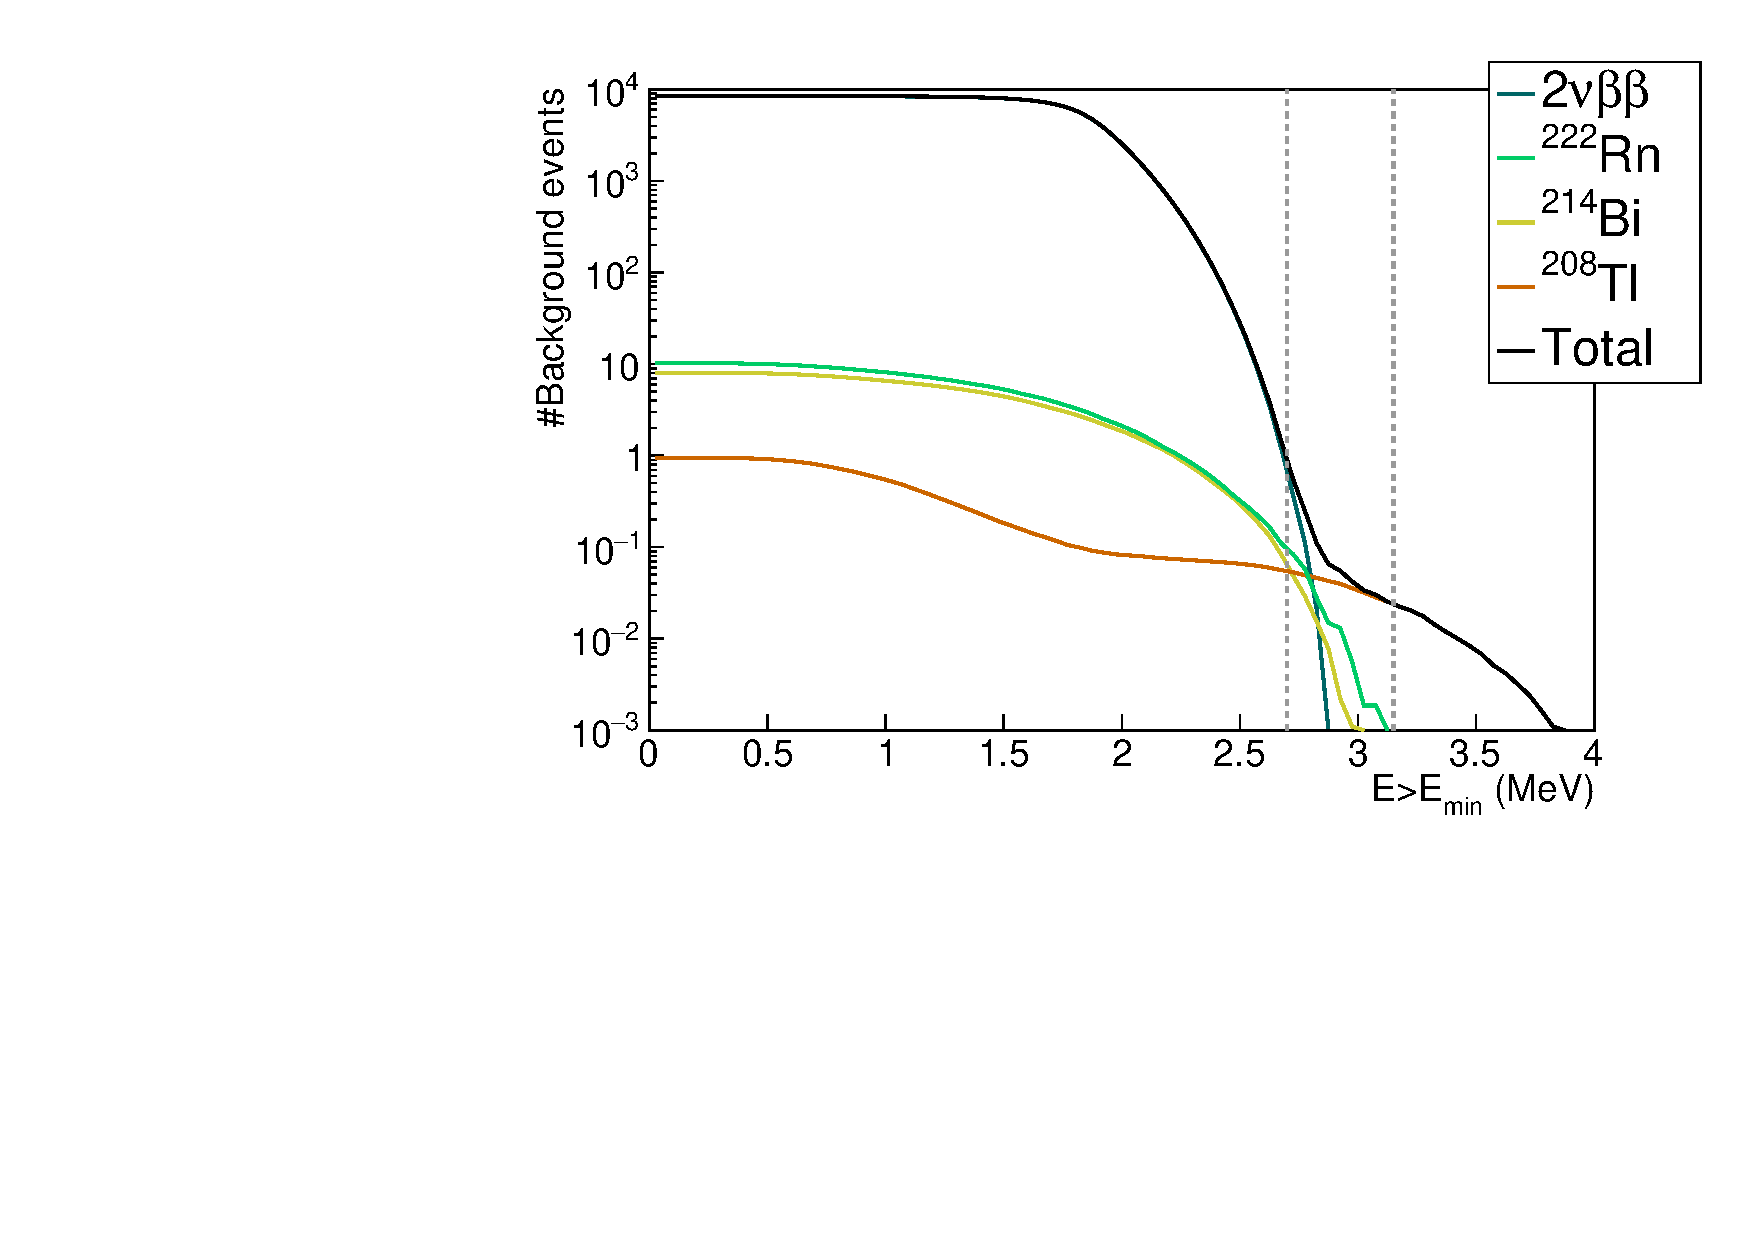
\includegraphics[width=1.1\textwidth]{Sensitivity/fig_sensitivity/Nbackground_spectrum_with_B_82Se.pdf}
  \captionsetup{justification=centering}
  \caption{
    \label{subfig:sensitivity_Nbkg_spectra}}
\end{subfigure}
\caption{(a) Efficiency spectra for $\text{E}>\text{E}_{\text{min}}$, for the $\zeronu$ signal and for the main backgrounds.
  (b) Expected number of background events, for $\text{E}>\text{E}_{\text{min}}$.
  \label{fig:Nbkg_eff_spectra}}
\end{figure}

%% Tab.~\ref{tab:2e_expected_counts} sums up the expected number of $2e$ topologies in the full energy range as well as in the region of interest.
%% \begin{table}[h]
%%   \centering
%%   \begin{tabular}{|c|c|c|}
%%     \hline
%%     & Full energy range & [$2.7$;$3.2$] MeV \\
%%     \hline\hline
%%     $\epsilon_{0\nu}$ (\%)  &  & $14.7$ \\
%%     $\twonu$  &  & $0.40$ \\
%%     \Tl  &  & $0.050$ \\
%%     \Bi  &  & $0.054$ \\
%%     \Rn  &  & $0.24$ \\
%%     \hline
%%   \end{tabular}
%%   \caption{Expected number of counts for the full energy range and for the region of interest.
%%   \label{tab:2e_expected_counts}}
%% \end{table}
%% To summarise, the total number of expected background events in the [$2.7$;$3.2$] energy range is $8.5 \times 10^{-5}$ keV$^{-1}$.kg$^{-1}$.y$^{-1}$.

The Feldman-Cousins statistics~\cite{art:feld-cous} is a wide-used method in rare events search experiments, providing confidence intervals for upper limits in the case of Poisson processes with background.
Given the expected number of background events, this method gives a limit on the number of expected signal events $N_{\text{expected}}$ , in a certain energy window, with a $90\%$ confidence interval.
As a consequence, the limit on $\Tbeta$ described in Eq.~\eqref{eq:tbeta_limit} is provided as a function of the lower energy bound $E_{\text{min}}$ and the upper energy bound $E_{\text{max}}$ of the considered energy range.
The region of interest held for the search of $\zeronu$ decay is the one maximising the limit on $\Tbeta$.
It depends on the exposure, on the isotope chosen for the experiment, as well as its total quantity inside the source foils, all of these different conditions being detailed in the following.
For the demonstrator exposure, with \Se\ sources, and a $25$ G magnetic field, the ROI is found to be [$2.7$;$3.2$] MeV.

Thereafter, we present and discuss the results obtain in the framework of this study, regarding different exposures (demonstrator and final detector), and different internal background activities (presented in Tab.~\ref{tab:real_target_act}).
Also, and this is the main purpose of this study, we discuss the influence of the presence of the magnetic field on the final detector's sensitivity.

\section{Magnetic field}

As detailed in Sec.~\ref{sec:magnetic_field}, the SuperNEMO demonstrator was originally designed with a copper coil, similarly to NEMO-$3$, delivering a magnetic field inside the tracker volume, aiming to provide an electron/positron discrimination by fitting the curved particle tracks by an helix.
Studies have been lead to evaluate its influence on the optical modules and on the event reconstruction~\cite{CalvezThesis}\cite{internal:magnetic_field}.


\subsection{Influence of the magnetic field on optical modules and reconstruction efficiency}

SuperNEMO PMTs are protected from the external magnetic field by an iron shield.
Unfortunately, the latter do not perfectly protect the PMTs, and a residual magnetic field is measured inside the shieldings, leading to charge losses and worsened energy resolution.
These studies showed that applying a $25$ G magnetic field, and protect the PMTs with iron magnetic shields would be optimal, but not without consequences.
In fact, for the recommended value of $25$ G for the magnetic field, PMT charge losses would be close to $8\%$, and the PMT energy resolution would be increased of $\sim 3\%$.
Moreover, the PMTs shieldings could themselves severely impact the shape of the field lines, as well as its strength, from the calorimeter wall to the source foil location: with a $25$ G magnetic field generated by the copper coil, barely $10$ G is expected near the source foils, and this value decreases quickly as we get closer to the calorimeter walls.
The reconstruction efficiency could therefore be greatly impacted:
the magnetic field intensity varying from the source foils to the calorimeter wall, electrons trajectory curvatures are not constant, and the track is less well fitted.
This effect is higher as the electron energy decreases.

Despite the fact that magnetic shields were designed and installed to protect the PMTs, this field can have a great impact on the calorimeter detection efficiency, and thus could degrade the detector's sensitivity to the $\zeronu$ decay.
If the studies cited have evaluated the influence of the presence of the magnetic field on the reconstruction efficiency of $\zeronu$ events, it remains to be seen its consequences on the final demonstrator sensitivity.

\subsection{Simulations of the magnetic field inside the demonstrator and reconstructed track fit}
In order to study the influence of the magnetic field on the SuperNEMO $\Tbeta$ sensitivity, the simulations and reconstructions of decays described in Sec.~\ref{sec:sensitivity_simus} have been performed in three different conditions:
\begin{itemize}
\item simulations where the magnetic field is turned off,
\item simulations with a $25$ G \emph{uniform} magnetic field (following recommendations \cite{CalvezThesis}),
\item simulations with a $25$ G \emph{mapped} magnetic field, taking into account more realistic variations of the magnetic field inside the detector~\cite{docdb:map_magnetic_field2015}.
\end{itemize}
Each magnetic field conditions have the same number of simulated events, as summed up in Tab.~\ref{tab:sensitivity_simulations}.
Depending on the case considered, the electrons will not have the same trajectory curvature: in the first no-field case, electron tracks are straight lines.
The fitting algorithm have thus be modified to match line trajectories.
In the second uniform-field case, the best track fit is performed by helices.
Finally, the best tracking option (line or helix) for the third mapped-field will be discussed in the next section.
%% \begin{figure}[h]
%% \centering
%% \begin{subfigure}[t]{0.48\textwidth}
%%   \centering
%%   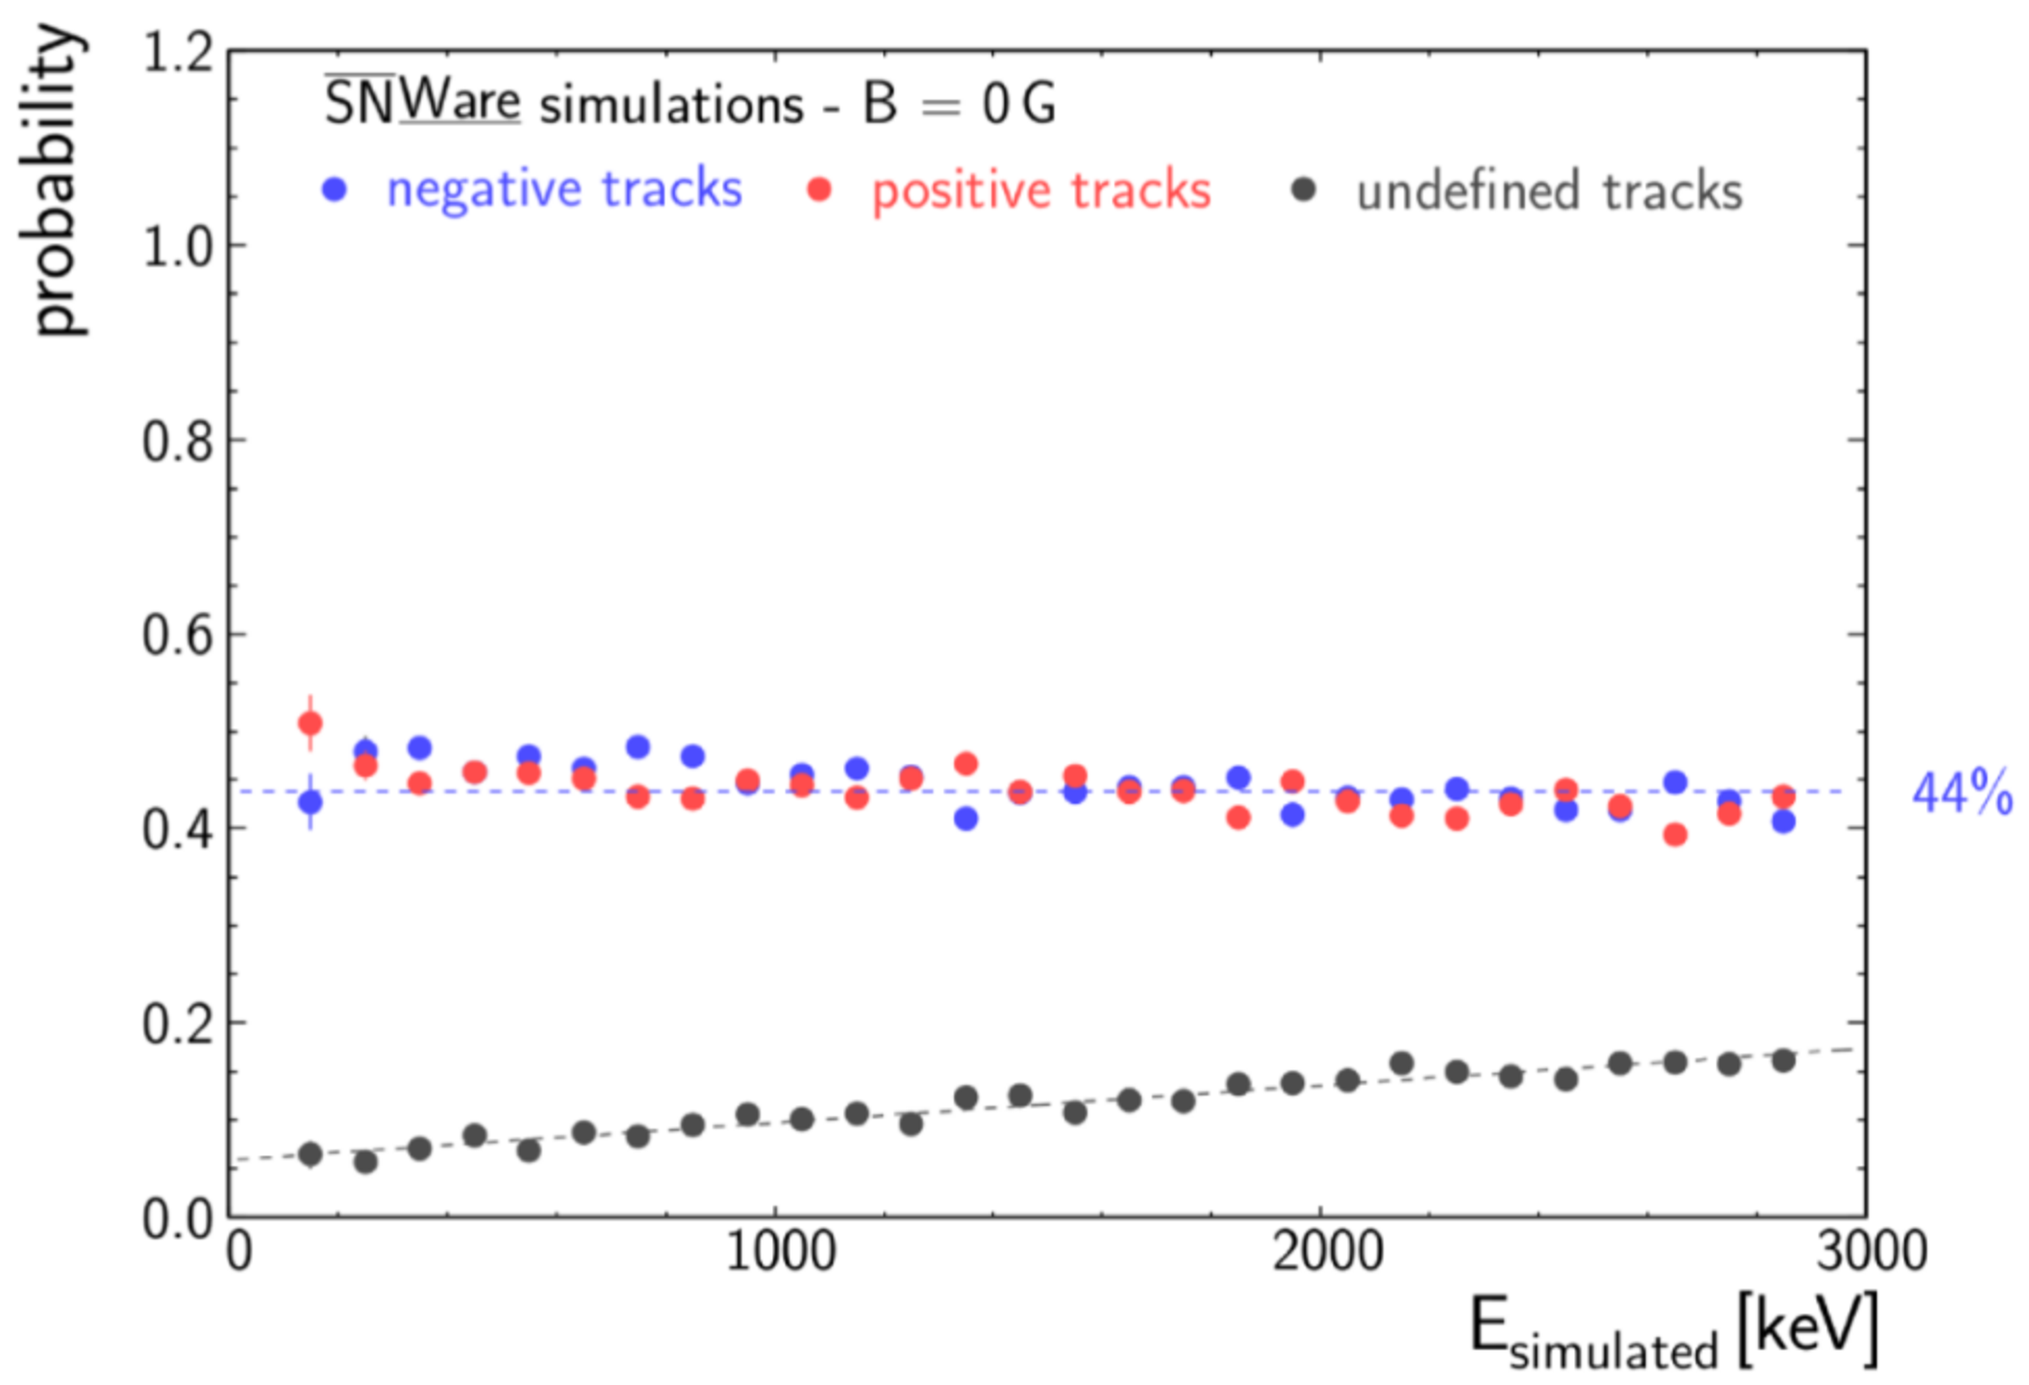
\includegraphics[width=1.\textwidth]{Sensitivity/fig_sensitivity/line_fitting.pdf}
%%   \captionsetup{justification=centering}
%%   \caption{
%%     \label{subfig:}}
%% \end{subfigure}
%% \hfill
%% \begin{subfigure}[t]{0.48\textwidth}
%%   \centering
%%   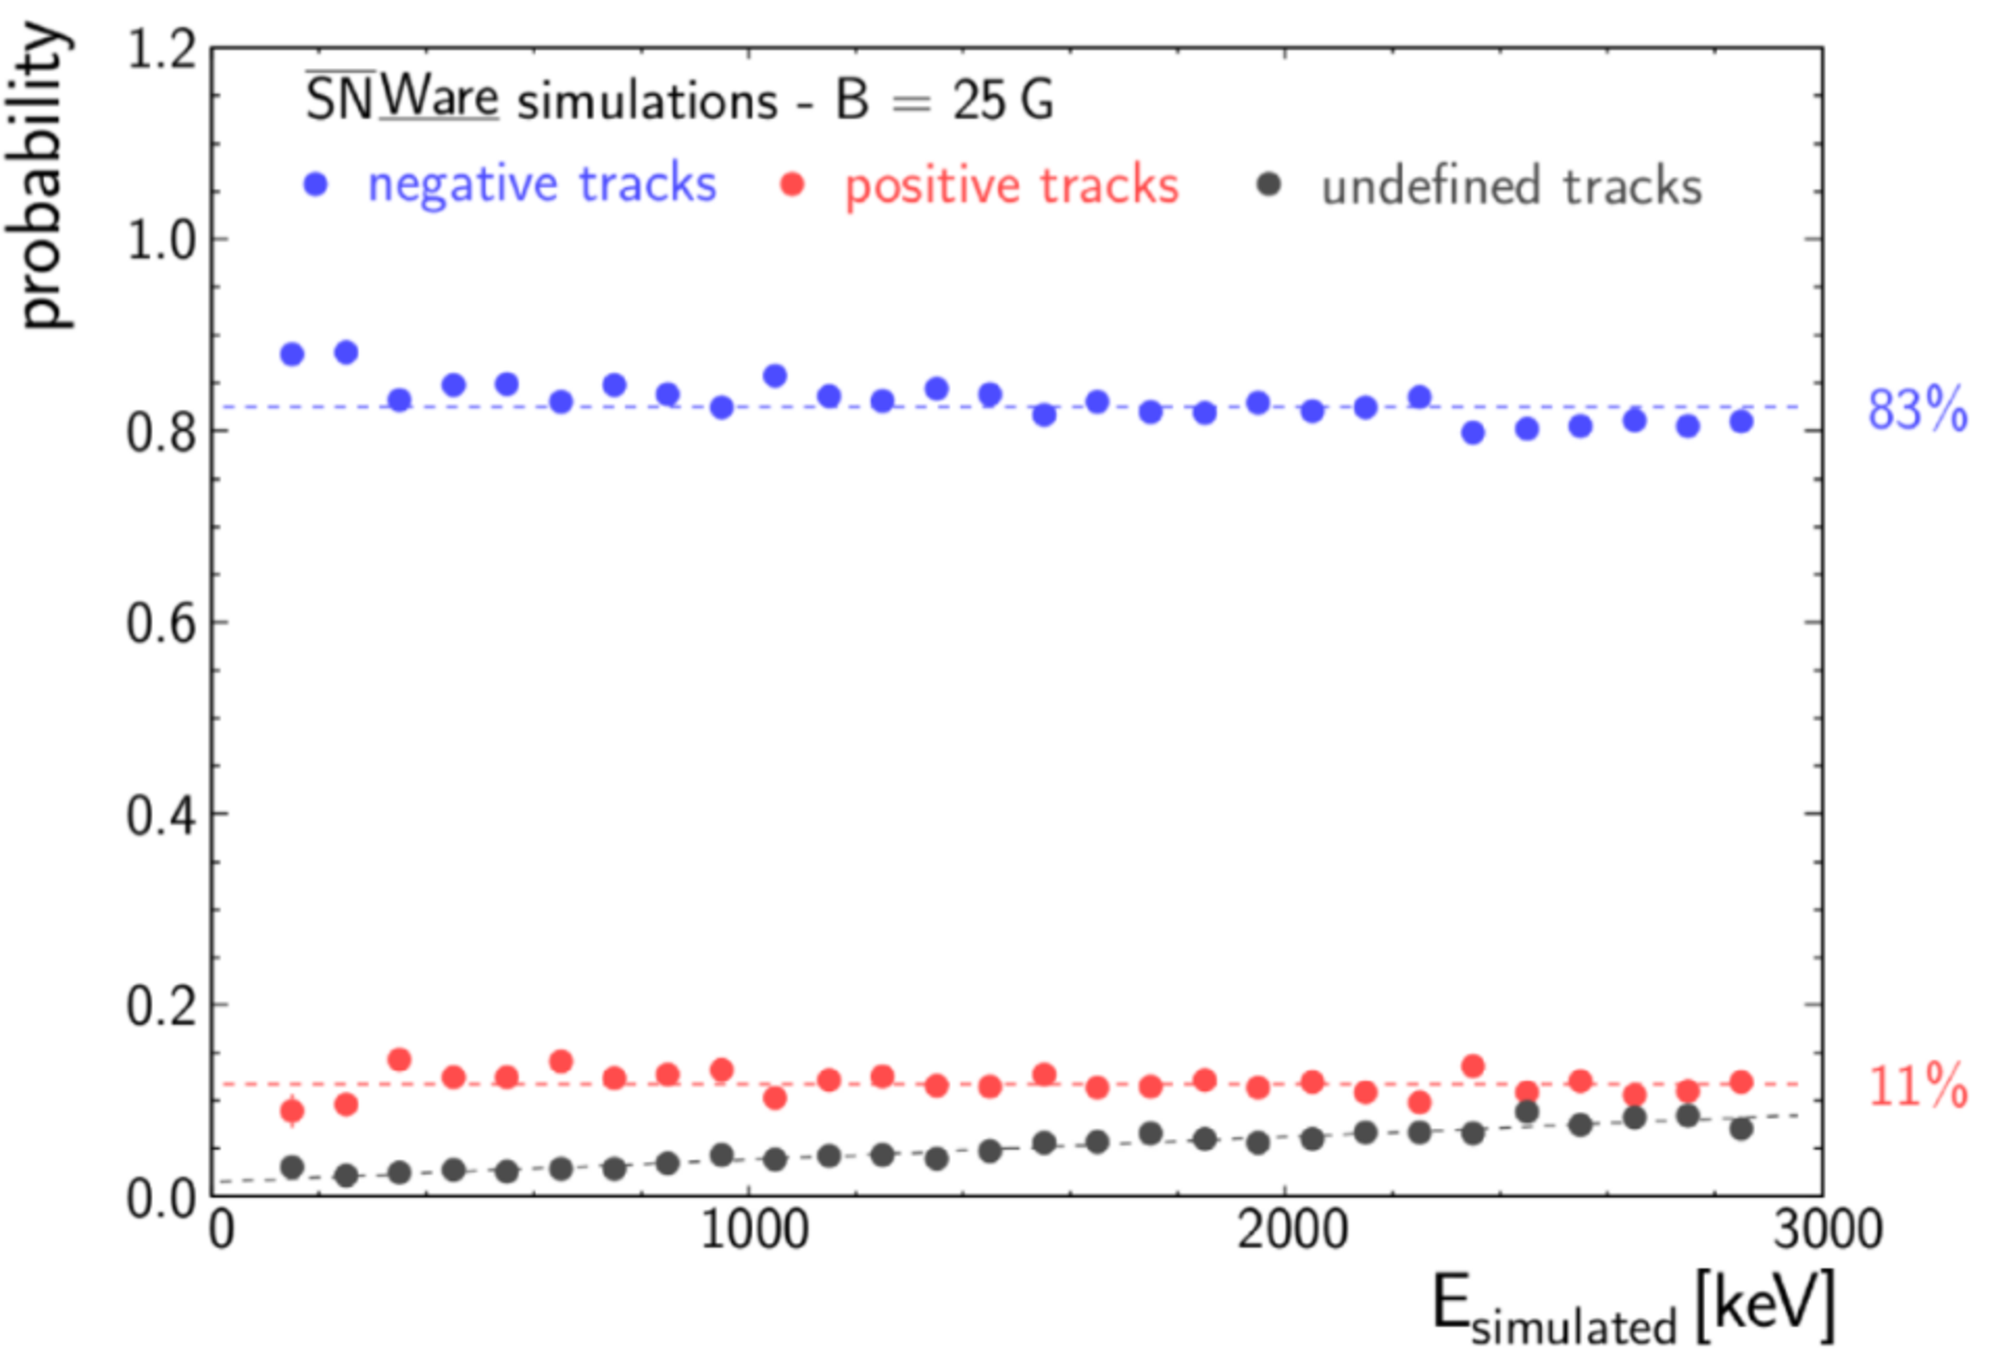
\includegraphics[width=1.\textwidth]{Sensitivity/fig_sensitivity/helix_fitting.pdf}
%%   \captionsetup{justification=centering}
%%   \caption{
%%     \label{subfig:}}
%% \end{subfigure}
%% \caption{Proportion of electrons reconstructed with a negative (blue), a positive (red) or an undefined charge (black) as a function of their simulated energy, in the absence of a magnetic field (a), and in a 25 G magnetic field (b).
%%   From~\cite{CalvezThesis}.
%%   \label{fig:track_fit}}
%% \end{figure}



\section{Demonstrator sensitivity to the $\zeronu$ decay}

The limit set on the $\Tbeta$ is given by Eq.~\eqref{eq:tbeta_limit}, and depends on the background level, in a way we will detail in this section.
One of the main goal of this study is also to determine the dependence of the sensitivity on the magnetic field applied inside de wire chamber.
In the following, we detail the results presented in Fig.~\ref{fig:real_target_act}, looking at one after another the influence of the contamination levels and the magnetic field on the sensitivity to the $\zeronu$ decay.
\begin{figure}[h]
  \centering
  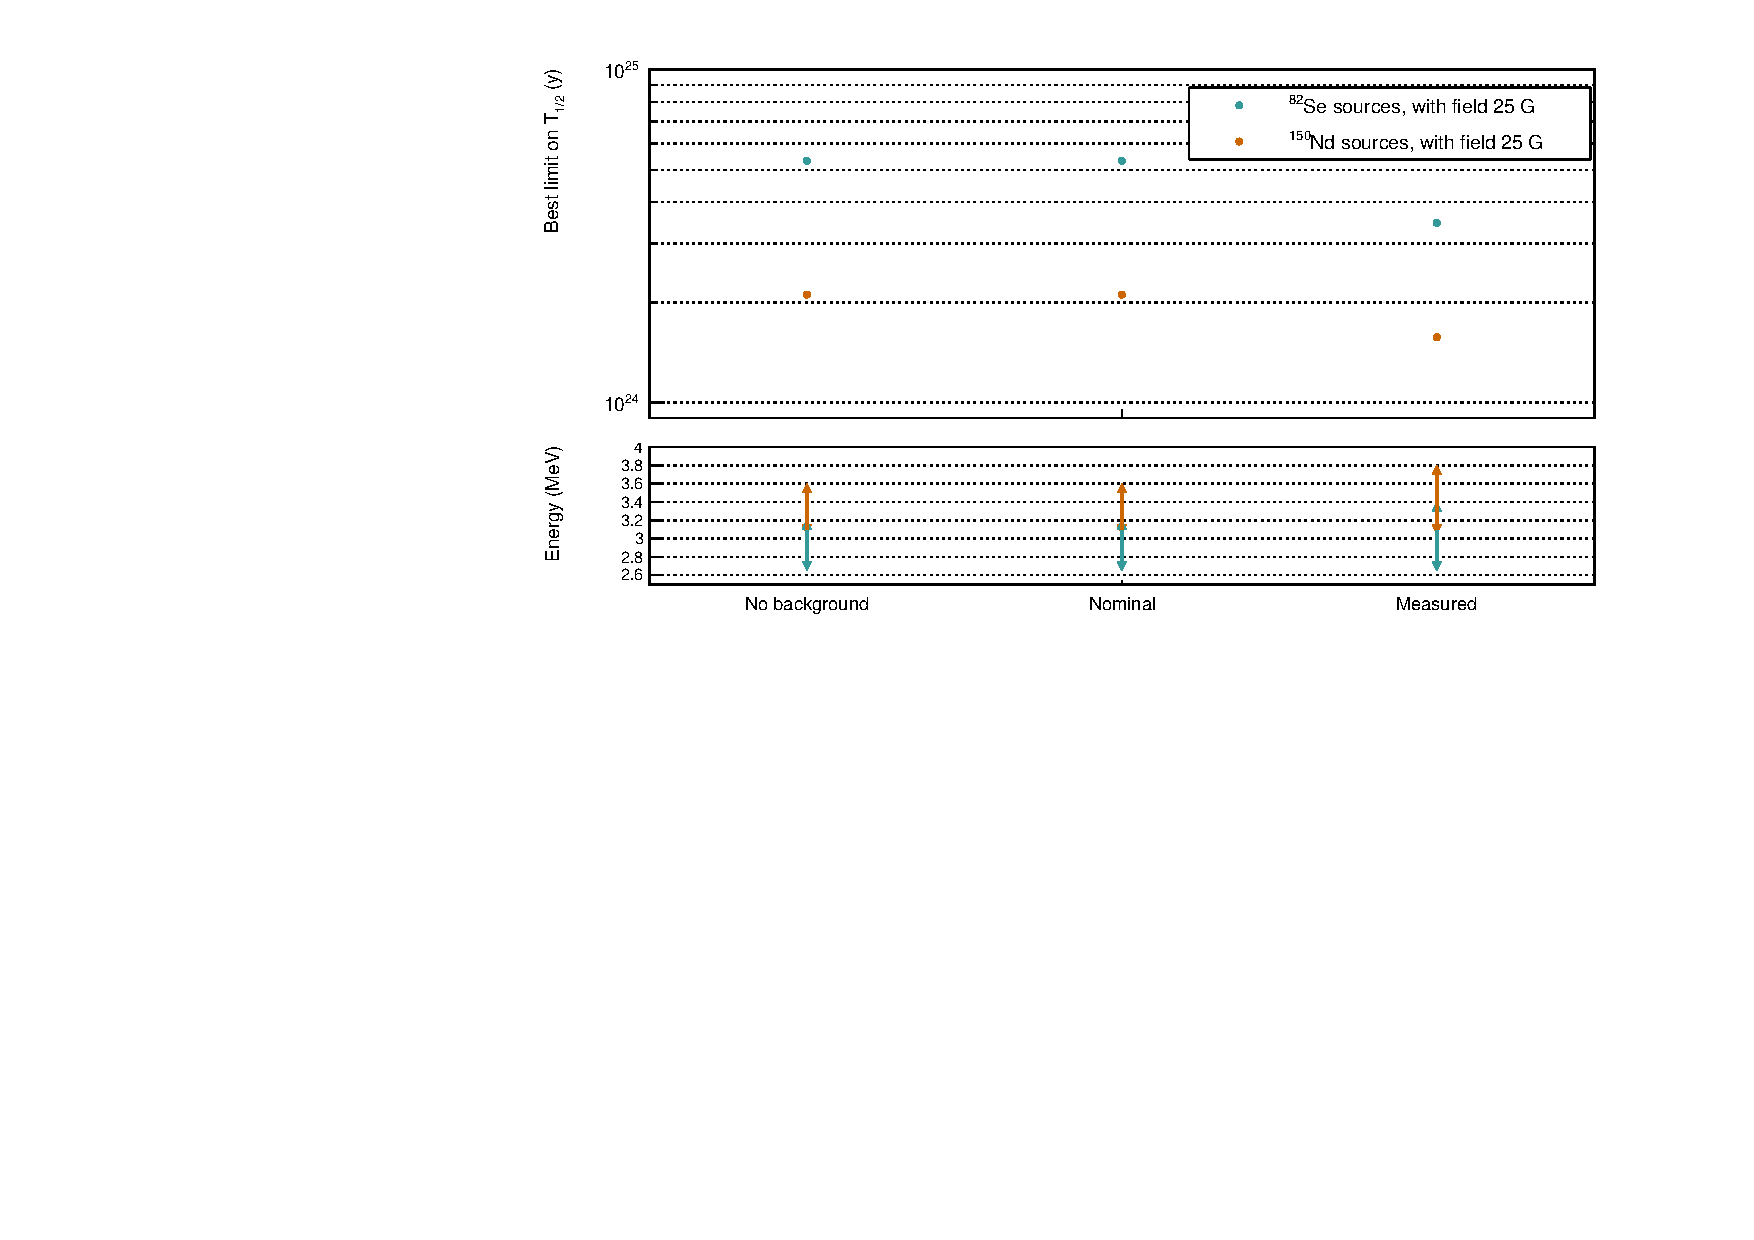
\includegraphics[width=1.1\textwidth]{Sensitivity/fig_sensitivity/contamination_level_Se.pdf}
  \caption{Best limit set on $\zeronu$ half-life (top pad), and the corresponding ROI (bottom pad), as a function of the contamination level considered.
    \label{fig:real_target_act}}
\end{figure}

\subsection{Influence of the contamination levels}

Target levels of contaminations inside the source foils and inside the wire chamber have been set to match the expectations on final detector's sensitivity to the $\zeronu$.
Preliminary measurements have been performed to determine the actual background contamination levels of the source foils, presented in Tab.~\ref{tab:real_target_act}.
In Fig.~\ref{fig:real_target_act}, three distinct levels of internal contaminations are considered: a hypothetical case where the source foils are non contaminated at all (the \emph{no background} case), and two realistic cases, where the targeted internal contamination levels are reached on one hand, and where the measured levels are applied on the other hand.

Let us first compare the two first, where no difference between the best $\Tbeta$ or the ROI is observed.
This is explained by the Feldman-Cousins statistics employed to determine the number of expected signal events, given the number of observed background events.
When the expected number of background events is negligible (which is the case here), the probability $p$ to observe $n_{s}$ events, expecting $s$ signal events is given by a Poisson distribution
\begin{equation}
p = \frac{e^{-s}s^{n_{s}}}{n_{s}!}\,.
\end{equation}
If no background event is observed - and this is assumed to put an upper half-life limit - then $p = e^{-s}$.
We can set an upper limit on the expected signal yield $s$ excluding values of $s$ for which $p < \alpha$, here considering $\alpha = 10\%$ ($1-\alpha = 90\%$ CL).
The upper limit for a negligible expected number of background and no signal events observed is therefore $s \leq 2.303$ ($90\%$ CL).
A direct consequence is, considering that the background levels for the two first cases are negligible, they both reach this limit on the expected number of signal events.

We focus now on the last case, where the measured levels of internal contaminations are used to determine the best limit on $\Tbeta$.
The levels of internal contaminations are no more negligible and influence the value of $\Tbeta$




\subsection{Influence of the magnetic field}
\begin{itemize}
\item avec variation coupure énergie\\
\item Parler du champ non uniforme/attenuation
\end{itemize}



\section{Final detector sensitivity}

the final goal of the SuperNEMO demonstrator is to demonstrate that the NEMO technology is scalable to reach high half-life sensitivity on the $\zeronu$ decay.
It was therefore mandatory to study the case of the final detector sensitivity, aiming to build $20$ modules like the SuperNEMO demonstrator, to reach imprecedented levels on $\mbb$ results.

\section{Other isotopes}

distribution t1/2 avec différents échantillons de simus (17.5 kg.y)

\section{Conclusion}
\begin{itemize}
\item Etude plus générale avec bkg externe+lab (reprendre chiffres NEMO3) + neutrons (cf NEMO3)
\item Plot général récap tous résultats
\item delayed cells->improvement, cf NEMO 3
\item ouverture sur possibilité d'étudier l'influence de la résolution en temps des PMs sur l'eff des coupures (Pint)
\end{itemize}
